\documentclass[thesis2.tex]{subfiles}

\begin{document}
\iffulldocument\else
	\chapter{Introduction}
\fi

\section{Historical Background}

Solitary waves are localized disturbances that maintain their shape as they propagate at a constant velocity. The first recorded observation of this phenomenon in nature is Russell's famous ``great solitary wave''. In 1834, the Scottish engineer John Scott Russell observed a ``large solitary elevation'' which arose when a barge stopped suddenly on the Union Canal near Edinburgh (see \cref{fig:canalwave} for a reenactment of this experiment in 1995). He was subsequently able to recreate the solitary wave experimentally, both in canals and in a wave tank in his backyard.  
\begin{figure}
\begin{center}
\includegraphics[width=7cm]{images/intro/solitonHW.jpg}
\caption[Solitary wave experiment]{Recreation of solitary wave experiment on the Union Canal, 12 July, 1995 \cite{Nature1995} }
\label{fig:canalwave}
\end{center}
\end{figure}

Although Russell published his results in 1845 \cite{russell1845}, his research was not well-received in the scientific community. The prominent mathematicians George Airy and George Stokes both rejected his work, as it did not agree with their results. The first mathematical theory to support Russell's observations was published by Boussinesq in 1872 \cite{Boussinesq1872}. Boussinesq opens his paper by vindicating Russell, stating that ``tous les ing{\'e}nieurs conaissent les belles exp{\'e}riences de J. Scott Russell... sur la production et la propagation des ondes solitaires'' [every engineer knows the great experiments of J. Scott Russell on the production and propagation of solitary waves]. In 1877, Boussinesq introduced an equation to describe solitary wave phenomena \cite{boussinesq1877essai}. This equation was rediscovered in 1985 by Diederek Korteweg and Gustav de Vries \cite{KdVoriginal} and is now known as the Korteweg-de Vries (KdV) equation. More recently, solitary waves have found applications in diverse fields, including fiber optics \cite{Taylor1992}, molecular systems \cite{Davydov1985}, Bose-Einstein condensates \cite{Panos2008BEC}, and ferromagnetics \cite{Kosevich1998}.

\section{Korteweg-de Vries equation}

The Korteweg-de Vries (KdV) equation is a prototypical model of an equation which admits solitary wave solutions. The equation derived by Korteweg and de Vries \cite{KdVoriginal} to describe wave propagation in a rectangular canal is  
\[
\frac{d \eta}{dt} = \frac{3}{2} \sqrt{\frac{g}{l}}
\frac{\partial}{\partial x}
\left( \frac{1}{2} \eta^2 + \frac{2}{3} \alpha \eta + \frac{1}{3} \sigma \frac{\partial^2 \eta}{\partial x^2}\right),
\]
where $\eta$ is the displacement above the surface, and remaning quantities are physical constants. It can be derived from the Euler equation for nonviscous, incompressible fluids, together with the appropriate boundary conditions and the assumption of irrotational flow \cite{SolitonPhysics}. With an appropriate change of variables, the KdV equation can be put into the more tractable form
\begin{equation}\label{KdV3}
\partial_t \phi + \partial_x^3 \phi - 6 \phi \partial_x \phi = 0
\end{equation}
This equation has been extensively studied since its introduction \cite{miles1981,drazin1989solitons,SolitonPhysics}, and many variants have been proposed. For wavespeed $c > 0$, an exact solitary wave solution to the KdV equation can be obtained by an inverse scattering transform.
\[
\phi (x,t)=-{\frac {c}{2}}\,\mathrm {sech} ^{2}\left({{\sqrt {c}} \over 2}(x-c\,t-a)\right),
\]
where $a$ is an arbitrary constant. The KdV equation also has another class of exact solutions which are periodic in nature. There are termed cnoidal waves, since they are expressed in terms of the Jacobi elliptic function $cn$ \cite{drazin1989solitons}. The cnoidal waves have sharper peaks and flatter troughs than ordinary sine waves. Both classes of solutions for water waves have been observed in nature, as shown in \cref{fig:waterwave}.
\begin{figure}
\begin{center}
\begin{tabular}{cc}
\includegraphics[width=7cm]{images/intro/beach.jpg} &
\includegraphics[width=7cm]{images/intro/cnoidal.jpg}
\end{tabular}
\caption[Solitary waves in nature]{Solitary wave observed off the coast of Hawaii \cite{ANDRIOPOULOS2009} (left), periodic solitary waves observed by US Army bombers near the Panama coast in 1933 (right) }
\label{fig:waterwave}
\end{center}
\end{figure}

Since solitary waves maintain their shape as they propagate at a constant velocity, they are equilibrium solutions to an approprate nonlinear PDE when written in a co-moving frame. For KdV, for example, a solitary wave with wavespeed $c$ is a solution to the third order ODE 
\begin{equation}\label{KdV3equilib}
\partial_x^3 \phi - c \partial_x \phi - 6 \phi \partial_x \phi = 0
\end{equation}
Since solitary waves are also localized, we can integrate equation \cref{KdV3equilib} once to get the second order ODE
\begin{equation}\label{KdV3eq}
\partial_x^2 \phi - c \phi - 3 \phi^2 = 0
\end{equation}

An alternative perspective on solitary waves comes from spatial dynamics, where the spatial variable $x$ is chosen as the evolutionary variable for a dynamical system. Using this approach, we can write \cref{KdV3eq} as a first order system in $x$ by letting $u = \phi$ and $v = \partial_x \phi$ to get
\begin{equation}\label{KdV3sd}
\begin{pmatrix}u \\ v
\end{pmatrix}'
= \begin{pmatrix}
v \\ c u + 3 u^3
\end{pmatrix}
\end{equation}
The origin is a hyperbolic saddle equilibrium with eigenvalues $\pm \sqrt{c}$. A solitary wave is a homoclinic orbit connecting the unstable and stable manifolds of this saddle. The cnoidal solutions are periodic orbits lying inside the homoclinic orbit.

Since the spatial dynamics of solitary wave solutions to KdV evolve in a two-dimensional phase space, they are constrained by the geometry of the plane. In particular, multi-pulse solitary waves, which correspond to multi-loop homoclinic orbits, cannot exist. Multi-pulses require a higher dimensional phase space in which to evolve, which in turn requires a higher dimensional ODE. A prototypical equation which exhibits multi-pulse solitary waves is the 5th order KdV equation (KdV5). When written in a co-moving frame with speed $c$, one form of KdV5 is
\begin{equation}\label{introKdV5}
u_t = u_{xxxxx} - u_{xxx} + c u_x - 2 u u_x .
\end{equation}
Localized, equilibrium solutions satisfy the fourth order ODE
\begin{equation}\label{introKdV5eq}
u_{xxxx} - u_{xx} + c u - u^2 = 0.
\end{equation}
Since the spatial dynamics of \cref{introKdV5eq} evolve in a four-dimensional space, a much greater diversity of solutions is possible than with KdV. In particular, multi-pulse homoclinic orbits are possible.

\section{Multi-pulses}

A multi-pulse is a multi-modal solitary wave which resembles multiple, well-separated copies of a single solitary wave. The study of multi-pulses goes back to at least the early 1980s, where Evans, Fenichel, and Faroe proved the existence of a double pulse traveling wave in nerve axon equations \cite{Evans1982}. A summary of early results related to multi-pulses can be found in \cite[Section 1]{Sandstede1998}. Existence of multi-pulse solutions to a family of Hamiltonian equations (which includes \cref{introKdV5eq}) was shown in \cite{Buffoni1996} using dynamics on the Smale horseshoe set. 

We will instead use the spatial dynamics approach due to Lin \cite{Lin1990} and Sandstede \cite{Sandstede1993,SandstedeStrut}. From this perspective, a multi-pulse is a homoclinic orbit which makes multiple loops but which stays close to a primary homoclinic orbit. Consider the general ODE
\begin{equation}\label{introgenODE}
U'(x) = F(U(x))
\end{equation}
for $U \in \R^{2n}$, where $F$ is smooth. This equation could arise, for example, from writing 
\cref{introKdV5eq} as a first-order system. Suppose further that 0 is a hyperbolic equilibrium for \cref{introgenODE}, and that there exists a homoclinic orbit $Q(x)$ which connects that hyperbolic equilibrium to itself. $Q(x)$ is the primary pulse solution, and lies in the intersection of the unstable manifold $W^u(0)$ and the stable manifold $W^s(0)$ of the equilibrium at 0. If equation \cref{introvareq} is derived from a PDE such as KdV or KdV5, $Q(x)$ is a solitary wave. We will assume that the primary pulse is nondegenerate, i.e. the intersection of the tangent spaces $T_{Q(x)}W^u(0)$ and $T_{Q(x)}W^s(0)$ is spanned by $Q'(x)$.

The linearization of \cref{introgenODE} about the homoclinic orbit $Q(x)$ is the variational equation
\begin{equation}\label{introvareq}
V'(x) = DF(Q(x)) V(x)
\end{equation}
Under the nondegeneracy assumption, $Q'(x)$ is the unique bounded solution to the variational equation, and there is a unique bounded solution $\Psi(x)$ to the adjoint variational equation
\begin{equation}\label{introadjvareq}
W'(x) = -DF(Q(x))^* W(x)
\end{equation}
which is perpendicular to $Q'(x)$. Furthermore, for all $x \in \R$, $\Psi(x)$ is perpendicular to the tangent spaces $T_{Q(x)}W^u(0)$ and $T_{Q(x)}W^s(0)$ of the unstable and stable manifolds. 

Heuristically, for a double pulse to occur, a solution must ``jump'' from the stable manifold at $x = L$ to the unstable manifold at $x = -L$. This is illustrated in the left panel of \cref{fig:wswu}.
\begin{figure}
\begin{center}
\begin{tabular}{cc}
\includegraphics[width=8cm]{images/intro/WsWu} &
\includegraphics[width=8cm]{images/intro/WsWuDouble}
\end{tabular}
\caption[Homoclinic orbit and double pulse]{Homoclinic orbit solution $Q(x)$ to \cref{introgenODE} (left panel). Double pulse solution (right panel). }
\label{fig:wswu}
\end{center}
\end{figure}
Suppose for simplicity that $U \in \R^4$ and the eigenvalues of $DF(0)$ are a quartet $\pm \alpha \pm \beta i$. Then the stable and unstable manifolds are both two-dimensional. Furthermore, the stable and unstable manifolds ``twist'' as they approach the equilibrium at 0, and the frequency of these twists is $2 \pi / \beta$. If equation \cref{introgenODE} is derived from an ODE such as \cref{introKdV5eq}, these ``twists'' are manifested as oscillations in the exponentially decaying tail of the solitary wave. A solution can only ``jump'' from the stable manifold at $x = L$ to the unstable manifold at $x = -L$ if the manifolds have the proper alignment, which is determined by these ``twists''. Specifically, write the tangent space to the unstable manifold as $T_{Q(x)}W^u(0) = \R Q'(x) \oplus Y^-(x)$, where $Y^-(x)$ is one-dimensional. For the ``jump'' to take place, $Q'(L)$ must be perpendicular to $Y^-(-L)$ \cite{Sandstede1993,Sandstede2002}. This is shown in \cref{fig:manifoldslineup}.
\begin{figure}
\begin{center}
\includegraphics[width=8cm]{images/intro/manifoldslineup}
\caption[Alignment of manifolds necessary for a double pulse]{Alignment necessary for a double pulse to exist. Primary homoclinic orbit is shown in red.}
\label{fig:manifoldslineup}
\end{center}
\end{figure}
Since $\Psi(-L)$ is perpendicular to $Y^-(-L)$, a double pulse solution exists when $Q'(L)$ is parallel to $\Psi(-L)$. A double pulse solution is illustrated by the purple line the right panel of \cref{fig:wswu}; in particular, note how it ``jumps'' from the stable manifold back to the unstable manifold near $x = L$.

The vectors $Q'(L)$ and $\Psi(-L)$ rotate in opposite directions with frequency $2 \pi/\beta$ as $L$ is varied, as shown in the left panel of \cref{fig:psiqrotate}. If $Q'(x)$ and $\Psi(-x)$ are parallel at $x = L$, then they will be parallel every quarter period, which is shown in the right panel of \cref{fig:psiqrotate}.
\begin{figure}
\begin{center}
\begin{tabular}{cc}
\includegraphics[width=8cm]{images/intro/psiqrotate} &
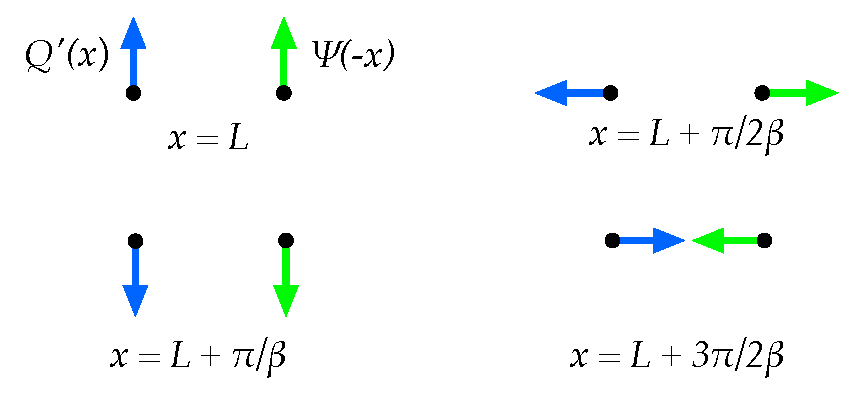
\includegraphics[width=8cm]{images/intro/psiqoneperiod}
\end{tabular}
\caption[Alignment of vectors necessary for a double pulse]{Rotation of $Q'(L)$ and $\Psi(-L)$ in opposite directions (left panel) Alignments of $Q'(x)$ and $\Psi(-x)$ every quarter period (right panel).}
\label{fig:psiqrotate}
\end{center}
\end{figure}
In half of the cases, $Q'(x)$ and $\Psi(-x)$ will be in the same direction, so that $\langle Q'(x), \Psi(-x) \rangle > 0$. In the other half of the cases, $Q'(x)$ and $\Psi(-x)$ will be in the opposite direction, so that $\langle Q'(x), \Psi(-x) \rangle < 0$. Since specific alignments of $Q'(L)$ and $\Psi(-L)$ are necessary for a double pulse to exist, double pulse solutions in general do not exist for all values of $L$ but only for a countable set of lengths $L$ indexed by an integer $m$ which represents the number of half-twists made by the stable and unstable manifolds \cite{SandstedeStrut}.  

To construct a multi-pulse, we will use a mathematical technique known as Lin's method, which is a Lyapunov-Schmidt reduction that allows us to find solutions near a known homoclinic orbit. This technique was introduced in \cite{Lin1990} and was used in \cite{Sandstede1993,SandstedeStrut} to construct multi-pulse solutions and \cite{Sandstede1998} to determine their spectral stability. Briefly, the method works as follows. For simplicity, we will state the procedure for a 2-pulse. We start with a known homoclinic orbit $Q(x)$ on $\R$. We then break the homoclinic orbit, either by varying a parameter in the system or by varying the initial conditions at $x = 0$. This yields a function $Q^-(x)$ on $\R^-$ which is contained in the unstable manifold and a function $Q^+(x)$ on $\R^+$ which is contained in the stable manifold. To construct a double pulse, we will ``reconnect'' these pieces using small remainder functions. Specifically, we will look for a double pulse solution as a piecewise function consisting of the four pieces
\begin{align*}
U_1^-(x) &= Q^-(x) + W_1^-(x) && x \in (-\infty, 0] \\
U_1^+(x) &= Q^+(x) + W_1^+(x) && x \in [0, L] \\
U_2^-(x) &= Q^-(x) + W_2^-(x) && x \in [-L, 0] \\
U_1^+(x) &= Q^+(x) + W_1^+(x) && x \in [L, \infty).
\end{align*}
which satisfies the matching condition at the pulse tails
\begin{equation}\label{introLin1}
U_1^+(L) = U_2^-(-L)
\end{equation} 
and the two matching conditions at the pulse centers
\begin{equation}\label{introLin2}
\begin{aligned}
U_1^-(0) &= U_1^+(0) \\
U_2^-(0) &= U_2^+(0)
\end{aligned}
\end{equation} 

The remainder functions $W_i^\pm(x)$ are the ``glue'' which reconnects $Q^-(x)$ and $Q^+(x)$ to form a double pulse. Lin's method allows us to find remainder functions $W_i^\pm(x)$ such that the first matching condition \cref{introLin1} is satisfied. In general, the matching conditions \cref{introLin2} are not satisfied. However, in most cases, the ``jumps'' $U_i^-(0) - U_i^+(0)$ can only occur in a direction which is perpendicular to the tangent spaces of the stable and unstable manifolds. For equation \cref{introgenODE}, it follows from the nondegeneracy assumption that these jumps at $x = 0$ can only occur in the direction of $\Psi(0)$. Projecting the jump $U_i^-(0) - U_i^+(0)$ onto $\Psi(0)$, we obtain two jump conditions
\begin{equation}\label{introLinJump}
\begin{aligned}
\xi_1 &= \langle \Psi(0), U_1^+(0) - U_1^-(0) \rangle \\
\xi_2 &= \langle \Psi(0), U_2^+(0) - U_2^-(0) \rangle.
\end{aligned}
\end{equation} 
A double pulse solution exists if and only if these two jump conditions are both 0. Thus we have reduced the problem of finding a double pulse solution to solving a system of two equations. This method is used in \cite{SandstedeStrut} to prove the existence of multi-pulse solutions to a class of equations which includes KdV5. 

\section{Outline of thesis}

We will present results on existence and spectral stability of multi-pulses in the following three Hamiltonian systems:
\begin{align*}
\partial_t u - \partial_x^5 u + \partial_x^3 u + 2 u \partial_x u &= 0 && \text{fifth-order Korteweg de-Vries equation (KdV5)} \\
\partial_t^2 u + \partial_x^4 u + \mathrm{e}^{u-1} - 1 &= 0 &&\text{Chen-McKenna suspension bridge equation} \\
i\partial_t u_n + d(u_{n+1} - 2 u_n + u_{n-1}) + |u_n|^2 u_n &= 0 &&\text{discrete nonlinear Schrodinger equation (dNLS)}
\end{align*}
KdV5 is a weakly nonlinear long wave approximation to capillary-gravity wave problem which also has applications to plasma physics and laser optics \cite{Pelinovsky2007}. Chen-McKenna is a smooth approximation to a model for waves propagating on an infinitely long suspended beam, and is motivated by observations of traveling waves on suspension bridges \cite{McKenna1990,Chen1997}. dNLS is the discrete analogue to the nonlinear Schr{\"o}dinger equation (NLS) and has applications to nonlinear optics and condensed matter physics \cite{Kevrekidis2009}.

The outline of the thesis is as follows. In \cref{chapter:chen}, we discuss the existence and spectral stabilty of multi-pulses in the Chen-McKenna suspension bridge equation. The stability analysis uses an extension of the Krein matrix, which is a tool that allows us to reduce the infinite dimensional eigenvalue problem to a finite dimensional one. In \cref{chapter:DNLS}, we perform a similar analysis for the discrete nonlinear Schr{\"o}dinger equation. In \cref{chapter:kdv5}, we introduce the 5th order KdV equation, discuss prior results, and present numerical results. From here, we turn to analysis. In \cref{chapter:kdv5general}, we formulate a generalization of the problem of interest, for which KdV5 is a specific case. In \cref{chapter:kdv5multi}, we discuss the existence and spectral stability of multi-pulse solutions to KdV5 as well as the existence of periodic multi-pulses. The proof for the existence of periodic multi-pulses is lengthy and is deferred to \cref{perexistproof}. We conclude with a brief chapter on future directions for research.

\iffulldocument\else
	\bibliographystyle{amsalpha}
	\bibliography{thesis2.bib}
\fi

\end{document}